\begin{figure*}
\centering
\begin{subfigure}{.18\textwidth}
  \centering
  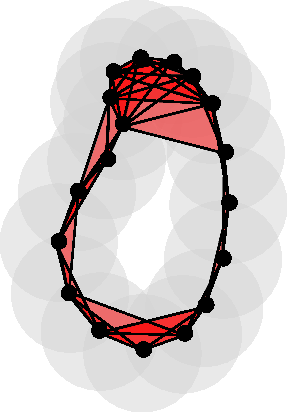
\includegraphics[width=.95\linewidth]{rips.pdf}
  \caption{$\Cech_r(X)$.}
\end{subfigure}
\hfill
\begin{subfigure}{.18\textwidth}
  \centering
  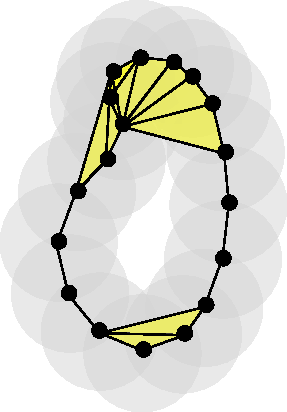
\includegraphics[width=.95\linewidth]{cechdelaunay.pdf}
  \caption{$\CechDel_r(X)$.}
\end{subfigure}
\hfill
\begin{subfigure}{.18\textwidth}
  \centering
  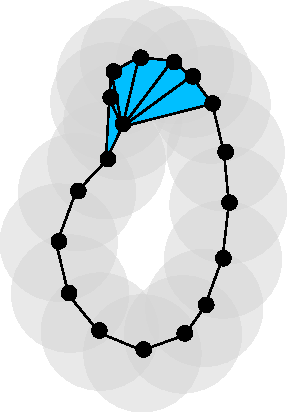
\includegraphics[width=.95\linewidth]{delaunay.pdf}
  \caption{$\Del_r(X)$.}
\end{subfigure}
\hfill
\begin{subfigure}{.18\textwidth}
  \centering
  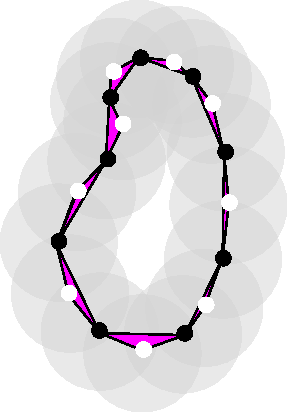
\includegraphics[width=.95\linewidth]{witness.pdf}
  \caption{$\Wit(L,W)$}
\end{subfigure}
\hfill
\begin{subfigure}{.18\textwidth}
  \centering
  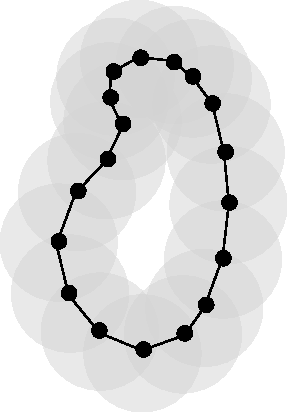
\includegraphics[width=.95\linewidth]{wrap.pdf}
  \caption{$\Wrap_r(X)$.}
\end{subfigure}
\caption{Four of five geometric complexes appearing in the collapsing sequence of the \v{C}ech-Delaunay Collapsing Theorem \ref{theo:collapse} from (a)-(c) and (e), according to \cite{bauer2017morse}. (a) A high dimensional \v{C}ech complex projected onto the plane. (b) The \v{C}ech-Delaunay complex, (c) the Delaunay complex, (d) the witness complex, which is an outlier in the row due to the changing shape by different witness sets (white bullets) and (e) the wrap complex.}
\label{fig:complexes}
\end{figure*}